
\documentclass{article}
\usepackage{mathtools, amssymb, amsthm, graphicx, ulem} % imports amsmath
\usepackage[a4paper, margin=1in]{geometry} % Set margins for better layout
\begin{document}
\sloppy
%vsechny pocty byly vypocitany pres python script -> soubor vypocty.py aby zajistena vyssi presnost

\section{První příklad zadání C}

\begin{figure}[!ht]
  \centering
  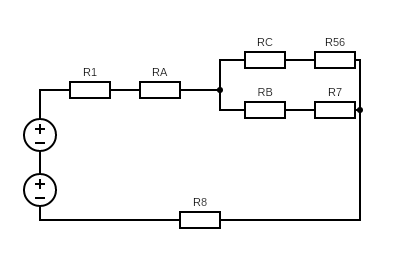
\includegraphics[width=0.9\textwidth, keepaspectratio]{/home/tjoslef/skola/zapisky/vut/IEL/projekt/priklad1a.png}
  \caption{Úprava pomocí hvězdy}
  \label{fig:hvezda}
\end{figure}

\[
    R_{56} = \frac{R_6 \times R_5}{R_6 + R_5}
\]

\begin{figure}[!ht]
  \centering
  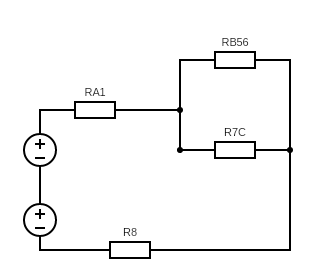
\includegraphics[width=0.9\textwidth, keepaspectratio]{/home/tjoslef/skola/zapisky/vut/IEL/projekt/priklad1b.png}
  \caption{Další úprava}
  \label{fig:dalsi_uprava}
\end{figure}


\[
R_{A1} = \frac{R_2 \cdot R_3}{R_2 + R_3 + R_4} + R_1
\]

\[
R_{B56} = \frac{R_2 \cdot R_4}{R_2 + R_3 + R_4} + \frac{R_6 \cdot R_5}{R_6 + R_5}
\]

\[
R_{C7} = \frac{R_3 \cdot R_4}{R_2 + R_3 + R_4} + R_7
\]

\[
R = \left(\frac{R_{B56} \cdot R_{C7}}{R_{B56} + R_{C7}}\right) + R_{A1} + R_8
\]

\[
I = \frac{U}{R}
\]

\[
U_{R3} = U - U_{R7} - U_{R1} - U_{R8}
\]

\[
U_{R7} = R_7 \cdot I
\]

\[
U_{R1} = R_1 \cdot I
\]

\[
U_{R3} = 3.6048
\]

\[
I_{R3} = \frac{U_{R3}}{R_3}
\]

\[
I_{R3} = 0.0190
\]
\clearpage
\section{Řešení druheho příkladu}
Úprava:

\begin{figure}[!ht]
  \centering
  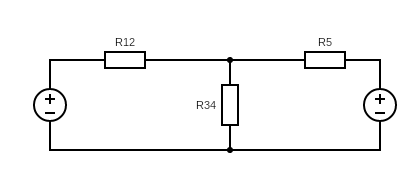
\includegraphics[width=0.9\textwidth, keepaspectratio]{/home/tjoslef/skola/zapisky/vut/IEL/projekt/priklad2.png}
  \caption{Další úprava}
  \label{fig:upravapriklad2}
\end{figure}

\[
    R_i = \frac{R_{12} \times R_5}{R_{12} + R_5}
\]
\[
    R_i = \frac{950 \times 80}{950 + 80} \quad \Rightarrow \quad R_i = 73.786
\]
\[
    I_x = \frac{U_2 - U_1}{R_{12} + R_5}
\]
\[
    I_x = \frac{180 - 130}{950 + 80} \quad \Rightarrow \quad I_x = 0.049
\]
\[
    U_i = U_1 + R_i \times I_x
\]
\[
    U_i = 130 + 950 \times 0.049
\]
\[
    I_{R34} = \frac{U_i}{R_i + R_{34}}
\]
\[
    \frac{176.55}{73.786 + 150} \quad \Rightarrow \quad I_{R34} = 0.789
\]
\[
    U_{R34} = 0.789 \times 150 \quad \Rightarrow \quad U_{R34} = 118.35 \, \text{V}
\]
\[
    U_{R4} = 118.35 \, \text{V}
\]
\[
    I_{R4} = \frac{118.35}{650} \quad \Rightarrow \quad I_{R3} = 0.1821 \, \text{A}
\]

\section{Reseni tretiho prikladu}
\[
    \text{Uzel A:} \quad \frac{130 - U_A}{47} + \frac{U_B -U_A}{28} - \frac{90 - (U_B - U_A)}{58} - \frac{U_A}{39} = 0
\]
\[
    \text{Uzel B:} \quad \frac{5}{10} + \frac{90 - (U_B - U_A)}{58} - \frac{U_B - U_A}{28} - \frac{U_B -U_C}{35} = 0
\]
\[
    \text{Uzel C:} \quad \frac{U_B - U_C}{35} - \frac{5}{10} - \frac{U_C}{25} = 0
\]
\[
    U_A = 43.9024 \, \text{V}
\]
\[
    U_{R2} = U_A  \quad \Rightarrow \quad U_{R2} = 43.9024 \, \text{V}
\]
\[
    I_{R2} = \frac{U_{R2}}{39} \quad \Rightarrow \quad I_{R2} = 1.1257 \, \text{A}
\]
\section{Reseni Ctvrteho prikladu}

\section{Reseni Pateho prikladu}
\begin{figure}[!ht]
  \centering
  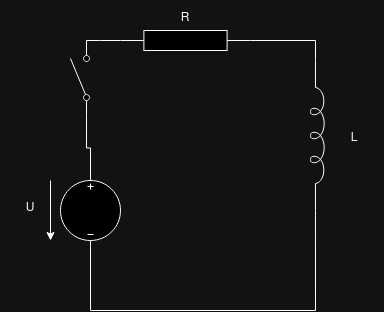
\includegraphics[width=0.9\textwidth, keepaspectratio]{/home/tjoslef/skola/zapisky/vut/IEL/projekt/paty_priklad.drawio.png}
  \caption{Paty priklad}
  \label{fig:priklad5}
\end{figure}
\subsection*{Z ceho budeme vychaze}
\[
i = \frac{U_r}{R} \quad \Rightarrow \quad \text{Ohmův zákon}
\]

\[
U_r + U_r = U \quad \Rightarrow \quad \text{Kirchhoffův druhý zákon}
\]

\[
i' = \frac{U_c}{L}, \quad i(0) = i_{L_0}
\]
\subsection*{Samotny vypocet}
\textbf{Kroky:}
1. Nejprve vyjádříme \( U_r \) z první rovnice.
2. Dosadíme \( U_r \) do druhé rovnice.
3. Poté dosadíme výsledek do třetí rovnice.

\[
i' = \frac{U}{L} - \frac{R}{L} \times i
\]

\textbf{Úprava:}

\[
L \times i' + R \times i = U
\]

\textbf{Charakteristická rovnice:}

\[
L\lambda + R = 0 \quad \Rightarrow \quad \lambda = \frac{-R}{L}
\]

\textbf{Očekávané řešení:}

\[
i(t) = I_L e^{\lambda t} \quad \Rightarrow \quad I_L(t) = I_L e^{\frac{-R}{L} t}
\]

\textbf{Dosadíme do upravené rovnice:}

\[
I_L'(t) = \frac{U}{L} e^{\frac{R}{L} t}
\]

\textbf{Jelikož se jedná o derivaci, musíme integrovat:}

\[
\frac{U}{L} \int e^{\frac{R}{L} t} \, dt
\]


\textbf{Substituce:} \( u = \frac{R}{L} t \quad \Rightarrow \quad du = \frac{R}{L} \, dt \)

\[
\frac{du}{dt} = \frac{R}{L}, \quad \text{takže} \quad dt = \frac{L}{R} du
\]

\[
\frac{U}{L} \int e^u \times \frac{L}{R} \, du
\]

\textbf{Zjednodušení:}

\[
\frac{U}{L} \times \frac{L}{R} \int e^u \, du
\]

\[
\frac{U}{R} e^u + C
\]


\textbf{Dosadíme zpět:}

\[
I_l = \frac{U}{R} + i(0) \time e^{\frac{R}{L} \times t}
\]
\[
    i(0) = _{LP} \rightarrow 8 - \frac{U}{R} = i(0)
\]

\[
    I_L = \frac{U}{R} + (8 - \frac{U}{R}) \times e^{\frac{R}{L} t}
\]
\[
I_L = \frac{1}{2} + \frac{15}{2} \times e^ {-5 \times t}
\]
graf prubehu:

\begin{figure}[!ht]
  \centering
  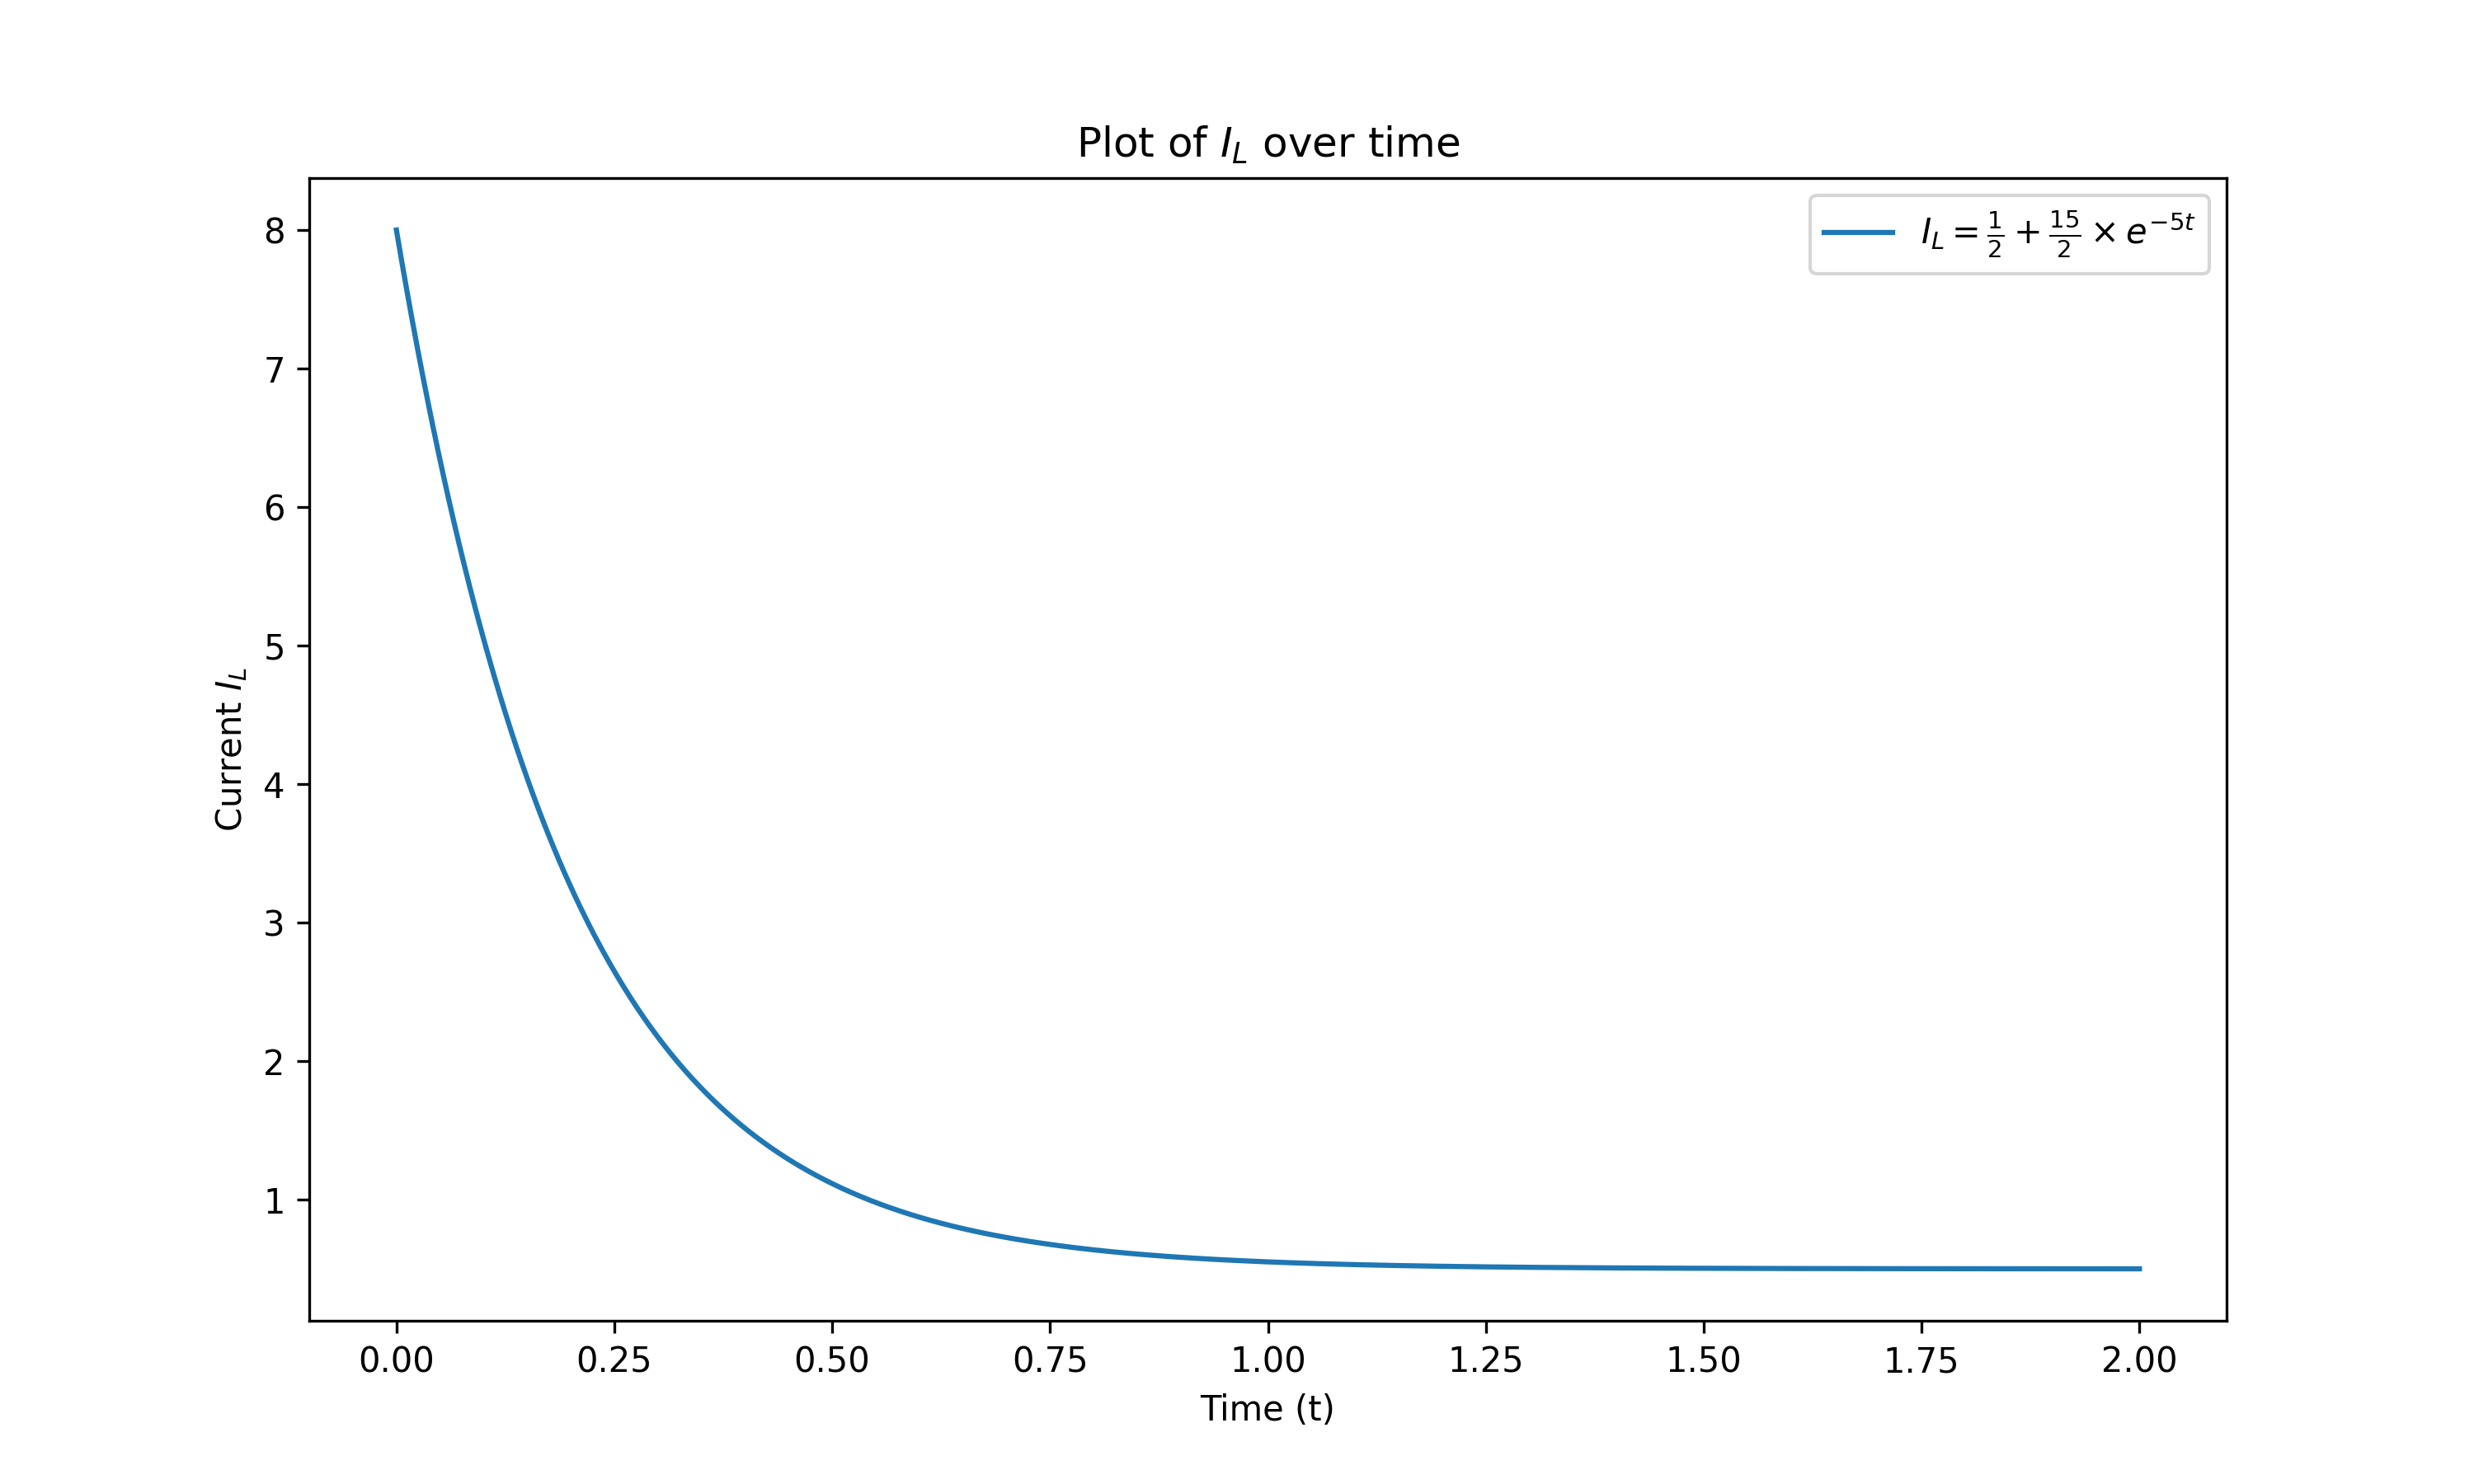
\includegraphics[width=0.9\textwidth, keepaspectratio]{/home/tjoslef/skola/zapisky/vut/IEL/projekt/graf5priklad.png}
  \caption{graf rovnice}
  \label{fig:graf prubehu}
\end{figure}
\end{document}




